\documentclass{recipe}

\begin{document}
\begin{recipe}{Pancakes}
  \servings{12}

  \begin{ingredients}
    \ingredient{4}{large}{eggs}
    \ingredient{\nicefrac{1}{4}}{packet}{yeast}
    \ingredient{\nicefrac{3}{4}}{stick}{butter}
    \ingredient{}{}{milk}
    \ingredient{}{}{butter}
    \ingredient{}{}{flour}
    \ingredient{}{}{sugar}
    \ingredient{}{}{baking powder}
    \ingredient{}{}{vanilla}
    \ingredient{}{}{salt}
  \end{ingredients}

  \begin{images}
    \begin{image}
      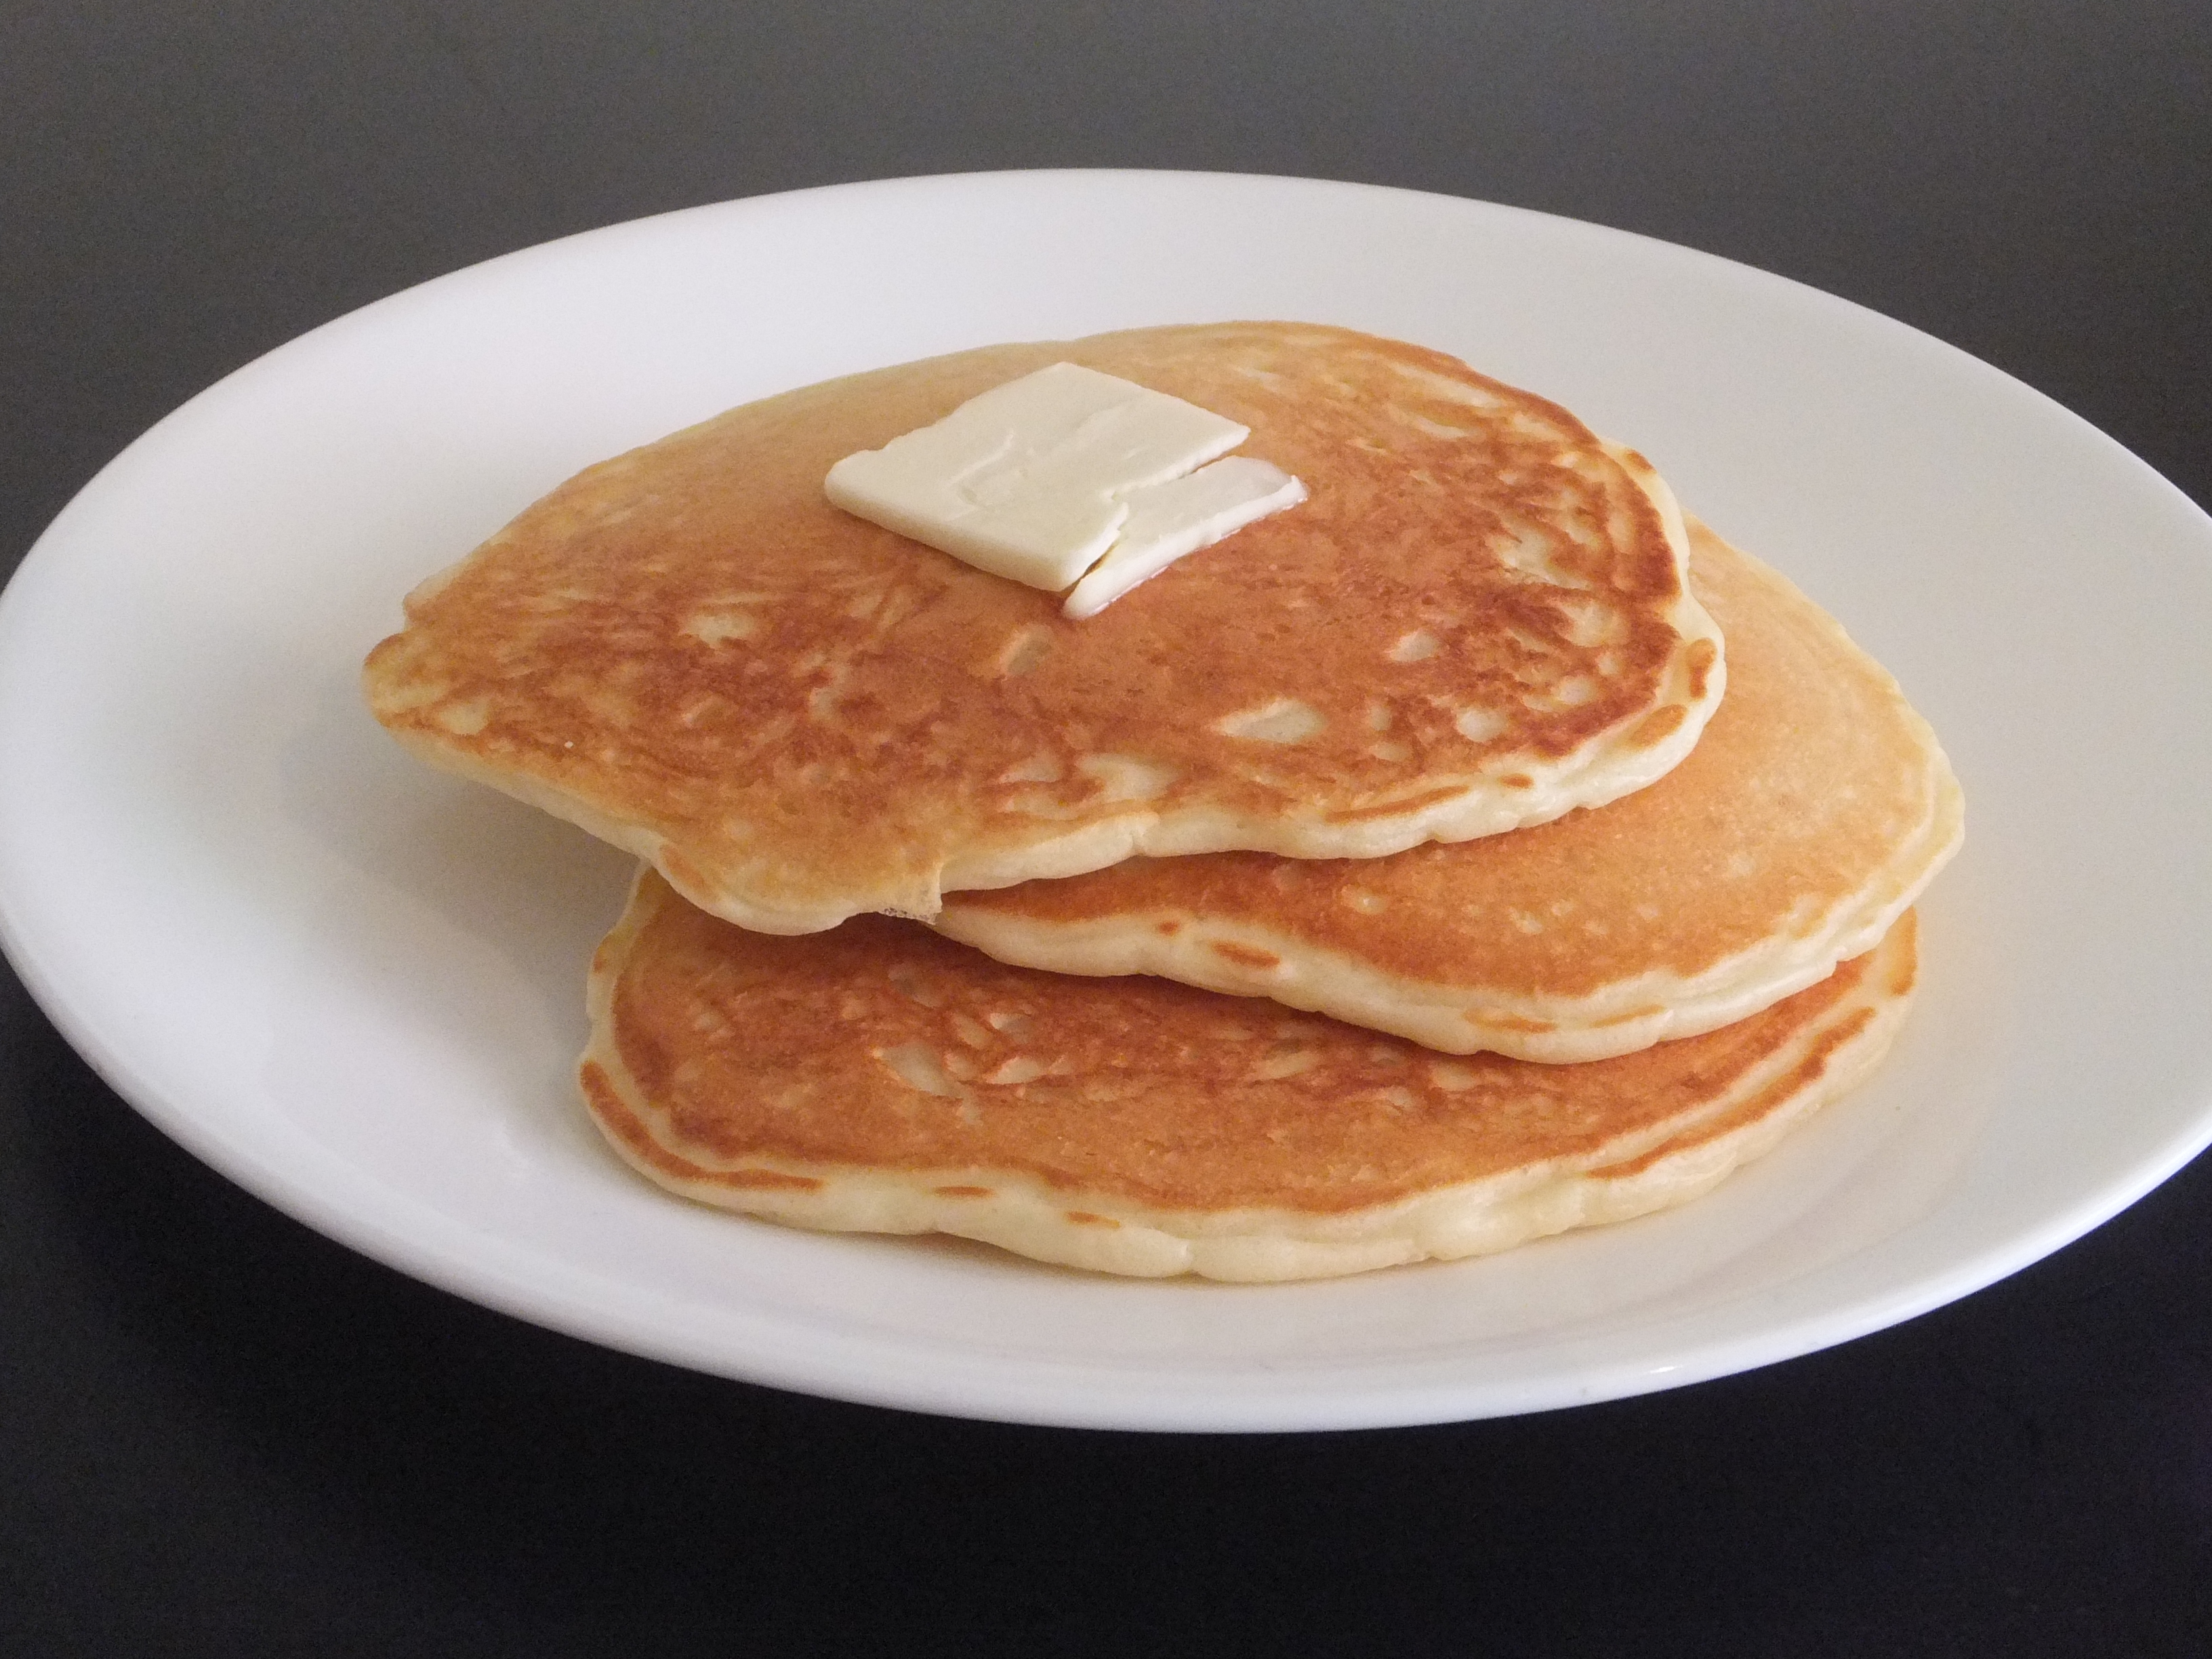
\includegraphics[width=\linewidth,trim=0px 0px 0px 0px, clip=true]{pancakes-01.jpeg}
    \end{image}
  \end{images}

  \begin{steps}
  \item Warm the milk and disolve the sugar and yeast in it.
  \item Cover and proof for a while.
  \item Mix in the eggs, butter, salt, and vanilla extract.
  \item Sift in the flour and baking powder.
  \item Let rise in the refrigerator overnight.
  \item Make pancakes!
  \end{steps}
\end{recipe}
\end{document}
